
\documentclass[11pt,a4paper]{article}

\usepackage[margin=1in]{geometry}
\usepackage[T1]{fontenc}
\usepackage{amsmath,amssymb}
\usepackage{booktabs}
\usepackage{array}
\usepackage{tikz}
\usepackage[hidelinks]{hyperref}
\usepackage{xcolor}
\usepackage{enumitem}

\title{\textbf{BCJRFormer ASIC Architecture}\\
\large Sequential Datapaths, FSMs and RTL Review Draft}
\author{Taimor Sabek \and Haiel Bader}
\date{\today}

\begin{document}

\maketitle

\section{Goal}

The first architecture step is to define the exact input/output boundary of the
\texttt{BCJRFormer} neural-network model used during inference. At this stage,
the internal transformer datapath is first introduced as a black box, then
expanded in the later architecture and RTL specification sections.

The scope of this document is therefore the software boundary of

\[
\texttt{BCJRFormer.forward}(y,\;padding\_mask)
\]

as implemented in the original BCJRFormer repository.

\section{Inference Boundary in the Repository}

During evaluation, the trainer invokes the model as

\begin{verbatim}
x_pred = self.model(y.to(self.device),
                    padding_mask.to(self.device))
\end{verbatim}

Therefore, the BCJRFormer model has two algorithmic inputs:

\begin{enumerate}[label=\arabic*.]
    \item \texttt{y} -- the windowed representation of the received sequences.
    \item \texttt{padding\_mask} -- identifies padded sequence positions.
\end{enumerate}

The model returns one output:

\begin{enumerate}[label=\arabic*.]
    \item \texttt{x\_pred} -- raw output logits of the BCJRFormer model.
\end{enumerate}

\section{First ASIC Black Box}

For the first ASIC architecture iteration, batch size is fixed to one.

\begin{center}
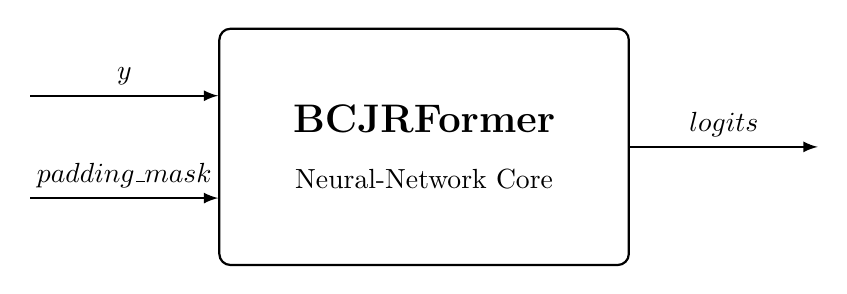
\begin{tikzpicture}[>=latex, thick]
    \node[
        draw,
        rounded corners,
        minimum width=5.2cm,
        minimum height=3.0cm,
        align=center
    ] (model) {\Large \textbf{BCJRFormer}\\[3mm]
               Neural-Network Core};

    \draw[->] (-5.0,0.65) -- (model.west |- 0,0.65)
        node[midway,above] {$y$};

    \draw[->] (-5.0,-0.65) -- (model.west |- 0,-0.65)
        node[midway,above] {$padding\_mask$};

    \draw[->] (model.east) -- (5.0,0)
        node[midway,above] {$logits$};
\end{tikzpicture}
\end{center}

This black box corresponds to the complete \texttt{BCJRFormer.forward()} function,
including the input embedding, positional/sequence embeddings, transformer
encoder, final linear projection, and the sequence-combination operation.

\section{Input 1: Windowed Received Data \texttt{y}}

The dataset first constructs a windowed representation with

\begin{verbatim}
y = self.trellis.get_windowed_version(...)
\end{verbatim}

Before batching, its shape is

\[
[M_{\max},\,N,\,W,\,S]
\]

and after the DataLoader adds the batch dimension,

\[
\boxed{
y \in \mathbb{R}^{1 \times M_{\max} \times N \times W \times S}
}
\]

where:

\begin{table}[h]
\centering
\begin{tabular}{>{\ttfamily}l p{9.5cm}}
\toprule
\textnormal{Parameter} & \textnormal{Meaning} \\
\midrule
M\_MAX & Maximum number of received sequences/transmissions. \\
N & Encoded sequence length / number of transformer positions per received sequence. \\
W & Trellis drift-window size. \\
S & Number of retained trellis-state features per window position. \\
\bottomrule
\end{tabular}
\end{table}

The trellis implementation defines

\[
S = q^{n_v}-1
\]

for the default non-full-state representation, and

\[
\texttt{WINDOW\_BLOCK\_DIM}
    = W \cdot S.
\]

At the beginning of \texttt{BCJRFormer.forward()}, the final two dimensions are
flattened. Thus the effective feature vector presented to the input embedding is

\[
\boxed{
y_{\mathrm{flat}}
\in
\mathbb{R}^{1 \times (M_{\max}N) \times (WS)}
}
\]

before projection to the transformer embedding dimension $d_{\mathrm{model}}$.

\section{Input 2: Padding Mask}

The dataset creates the padding mask from the padded entries of \texttt{y}.
For batch size one,

\[
\boxed{
padding\_mask
\in
\{0,1\}^{1 \times M_{\max} \times N}
}
\]

The model reshapes this mask internally for use by the transformer encoder.

Its purpose is to prevent padded positions, which correspond to unavailable
received sequences, from contributing to the model result.

\section{Output: Raw Logits}

The transformer output is projected by the final linear layer. For the binary
case ($q=2$), the model uses one output channel per encoded position.

After the outputs of the available received sequences are combined, the
BCJRFormer model returns

\[
\boxed{
logits
\in
\mathbb{R}^{1 \times N}
}
\]

for batch size one.

These values are \textbf{raw logits}. They are not yet decoded binary values.

\section{Sigmoid and Hard Decision}

During evaluation, the repository performs

\begin{verbatim}
x_pred = torch.round(torch.sigmoid(x_pred))
\end{verbatim}

\textbf{after} the call to \texttt{BCJRFormer.forward()}.

Therefore, for the first ASIC black box defined in this document,

\[
\boxed{\text{sigmoid and round are outside the BCJRFormer core}}
\]

and the output of the black box remains the raw logit vector.

For a later complete decoder architecture, the binary hard decision can be
implemented without explicitly calculating the sigmoid because

\[
\sigma(x) > 0.5
\iff
x > 0.
\]

Thus,

\[
\operatorname{round}(\sigma(x))
=
\begin{cases}
1, & x > 0,\\
0, & x \le 0.
\end{cases}
\]

This possible hardware optimization is not part of the current black-box
definition.

\section{Generic Architecture Parameters}

The first architecture can therefore be parameterized by:

\begin{table}[h]
\centering
\begin{tabular}{>{\ttfamily}l p{9.5cm}}
\toprule
\textnormal{Parameter} & \textnormal{Description} \\
\midrule
M\_MAX & Maximum number of received sequences. \\
N & Encoded sequence length. \\
WINDOW\_SIZE & Trellis window size $W$. \\
N\_STATE\_FEATURES & Number of state features $S$. \\
WINDOW\_BLOCK\_DIM & Input feature dimension $W \times S$. \\
D\_MODEL & Transformer embedding dimension. \\
NUM\_HEADS & Number of attention heads. \\
NUM\_LAYERS & Number of transformer decoder/encoder blocks used by the model. \\
Q & Symbol alphabet size; the first hardware target is $Q=2$. \\
\bottomrule
\end{tabular}
\end{table}

The concrete values will later be configured to match the trained reference
model and its golden Python results.

\section{Current Black-Box Interface Summary}

For the initial binary, batch-size-one architecture:

\[
\boxed{
\begin{aligned}
y &: [1,M_{\max},N,W,S] \\
padding\_mask &: [1,M_{\max},N] \\
BCJRFormer(y,padding\_mask) &\longrightarrow logits:[1,N]
\end{aligned}
}
\]



\section{Stage 2: Internal BCJRFormer Blocks}

After defining the BCJRFormer as a single black box, we now open the model one
level and identify its main internal blocks. At this stage, the goal is only to
define the architectural hierarchy; numerical precision and detailed datapaths
are left for later stages.

The BCJRFormer core can be represented as

\[
y
\rightarrow
\text{Input Embedding}
\rightarrow
\text{Position/Sequence Embedding}
\rightarrow
\text{Transformer Encoder}
\rightarrow
\text{Final Linear Layer}
\rightarrow
\text{Sequence Aggregation}
\rightarrow
\text{Logits}.
\]

The padding mask is used by the transformer and by the final sequence
aggregation.

\begin{center}
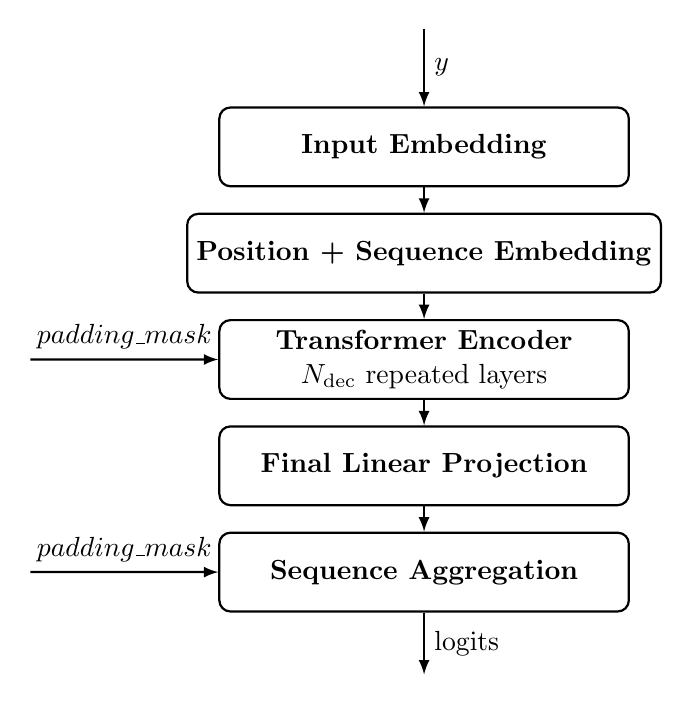
\begin{tikzpicture}[
    >=latex,
    thick,
    block/.style={
        draw,
        rounded corners,
        minimum width=5.2cm,
        minimum height=1.0cm,
        align=center
    },
    node distance=1.35cm
]
\node[block] (emb) {\textbf{Input Embedding}};
\node[block, below of=emb] (pos) {\textbf{Position + Sequence Embedding}};
\node[block, below of=pos] (tr) {\textbf{Transformer Encoder}\\$N_{\mathrm{dec}}$ repeated layers};
\node[block, below of=tr] (fc) {\textbf{Final Linear Projection}};
\node[block, below of=fc] (agg) {\textbf{Sequence Aggregation}};

\draw[->] (0,1.5) -- (emb.north) node[midway,right] {$y$};
\draw[->] (emb) -- (pos);
\draw[->] (pos) -- (tr);
\draw[->] (tr) -- (fc);
\draw[->] (fc) -- (agg);
\draw[->] (agg.south) -- (0,-6.7) node[midway,right] {logits};

\draw[->] (-5,-2.7) -- (tr.west)
    node[midway,above] {$padding\_mask$};
\draw[->] (-5,-5.4) -- (agg.west)
    node[midway,above] {$padding\_mask$};
\end{tikzpicture}
\end{center}

\subsection{Transformer Encoder}

The transformer encoder consists of $N_{\mathrm{dec}}$ repetitions of the same
self-attention layer:

\[
X_0
\rightarrow
\boxed{\text{Self-Attention Layer}}
\rightarrow
\boxed{\text{Self-Attention Layer}}
\rightarrow \cdots \rightarrow
\boxed{\text{Self-Attention Layer}}
\rightarrow X_{N_{\mathrm{dec}}}.
\]

Therefore, from an ASIC point of view, the repeated self-attention layer is the
main computational building block of the transformer core.

\subsection{Inside One Self-Attention Layer}

One transformer layer has two main branches:

\begin{enumerate}
    \item LayerNorm $\rightarrow$ Multi-Head Self-Attention $\rightarrow$
    Residual Addition.
    \item LayerNorm $\rightarrow$ Feed-Forward Network $\rightarrow$
    Residual Addition.
\end{enumerate}

This is a pre-normalization transformer structure.

\begin{center}
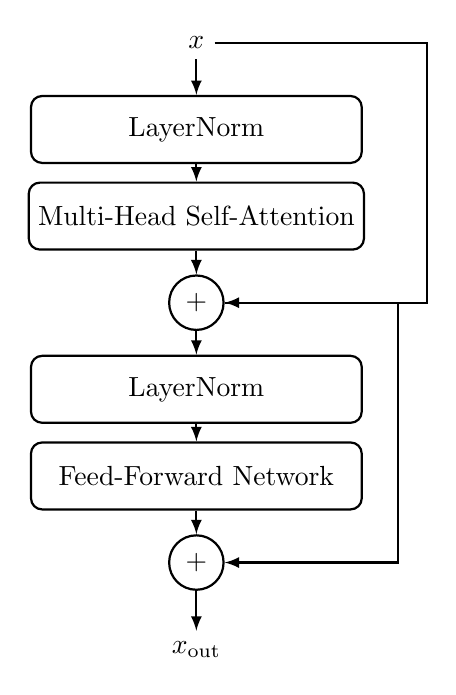
\begin{tikzpicture}[
    >=latex,
    thick,
    block/.style={
        draw,
        rounded corners,
        minimum width=4.2cm,
        minimum height=0.85cm,
        align=center
    },
    node distance=1.10cm
]
\node (xin) {$x$};
\node[block, below of=xin] (ln1) {LayerNorm};
\node[block, below of=ln1] (mha) {Multi-Head Self-Attention};
\node[circle,draw,below of=mha,minimum size=0.55cm] (add1) {$+$};
\node[block, below of=add1] (ln2) {LayerNorm};
\node[block, below of=ln2] (ffn) {Feed-Forward Network};
\node[circle,draw,below of=ffn,minimum size=0.55cm] (add2) {$+$};
\node[below of=add2] (out) {$x_{\mathrm{out}}$};

\draw[->] (xin) -- (ln1);
\draw[->] (ln1) -- (mha);
\draw[->] (mha) -- (add1);
\draw[->] (add1) -- (ln2);
\draw[->] (ln2) -- (ffn);
\draw[->] (ffn) -- (add2);
\draw[->] (add2) -- (out);

\draw[->] (xin.east) -- ++(2.7,0) |- (add1.east);
\draw[->] (add1.east) -- ++(2.2,0) |- (add2.east);
\end{tikzpicture}
\end{center}

\subsection{Multi-Head Self-Attention}

The multi-head attention block first produces the query, key, and value
representations:

\[
Q=XW_Q^T+b_Q,\qquad K=XW_K^T+b_K,\qquad V=XW_V^T+b_V.
\]

For each attention head, the core operation is

\[
A=
\operatorname{softmax}
\left(
\operatorname{masked\_fill}\left(\frac{QK^T}{\sqrt{d_k}},\mathrm{mask},-10^9\right)
\right),
\]

followed by

\[
Z=AV.
\]

The outputs of all heads are concatenated and passed through a final output
projection $W_O$ with bias $b_O$: $O=ZW_O^T+b_O$. Here weight matrices
follow the software storage convention $[\mathrm{out},\mathrm{in}]$.
The current padding mask broadcasts over query rows. The full RTL draft
below preserves this behavior explicitly and flags alternative key masking
as an algorithm change requiring review.

At the block level:

\[
X
\rightarrow
\{W_Q,W_K,W_V\}
\rightarrow
QK^T
\rightarrow
\text{Scaling + Mask + Softmax}
\rightarrow
AV
\rightarrow
\text{Concatenate Heads}
\rightarrow
W_O.
\]

Thus, the attention block contains four learned linear projections:
$W_Q$, $W_K$, $W_V$, and $W_O$.

\subsection{Feed-Forward Network}

The feed-forward network is composed of two linear transformations separated by
a GELU activation:

\[
d_{\mathrm{model}}
\rightarrow
4d_{\mathrm{model}}
\rightarrow
d_{\mathrm{model}}.
\]

Equivalently,

\[
x
\rightarrow
\text{Linear}
\rightarrow
\text{GELU}
\rightarrow
\text{Linear}
\rightarrow
y.
\]

Dropout exists in the software model but is disabled during inference, and
therefore does not require a dedicated arithmetic block in the inference ASIC.

\subsection{Architecture Hierarchy}

The current architecture decomposition is therefore:

\begin{itemize}
    \item \textbf{Level 0:} Complete BCJRFormer black box.
    \item \textbf{Level 1:} Input Embedding, Position/Sequence Embedding,
    Transformer Encoder, Final Linear Projection, and Sequence Aggregation.
    \item \textbf{Level 2:} Transformer Encoder =
    $N_{\mathrm{dec}}$ repeated Self-Attention Layers.
    \item \textbf{Level 3:} Each Self-Attention Layer =
    LayerNorm, Multi-Head Self-Attention, residual addition,
    LayerNorm, Feed-Forward Network, residual addition.
    \item \textbf{Level 4:} Multi-Head Self-Attention =
    $Q/K/V$ projections, scaled dot-product attention, masking,
    softmax, value multiplication, head concatenation, and output projection.
\end{itemize}




\section{Stage 2 Hardware View: Position + Sequence Embedding}

The second BCJRFormer block receives the embedded token vector from Stage 1 and
adds two learned vectors:

\[
x'_{m,n}=x_{m,n}+P[n]+E[m].
\]

Here, $P[n]$ is the learned positional embedding for encoded position $n$, and
$E[m]$ is the learned sequence embedding identifying received sequence $m$.

Both tables are model parameters learned during training and saved in the
model checkpoint, just like the linear-layer weights. In the code,
\texttt{pos\_embed} stores the positional table with shape
$[N,d_{\mathrm{model}}]$, and \texttt{seq\_embed.weight} stores the sequence
table with shape $[M_{\max},d_{\mathrm{model}}]$.

Before inference, the trained tables must be loaded into the corresponding
parameter memories. During inference, the controller uses $n$ and $m$ as
addresses to read the stored vectors. It does not calculate or train these
vectors from the received data. The calculation in this stage is the vector
addition $x'[m,n]=x[m,n]+P[n]+E[m]$. The software's
\texttt{sequence\_to\_embed} constructs sequence indices, not embedding values.

The block therefore contains two embedding memories and two vector-add
operations:

\[
x[m,n]
\rightarrow
\boxed{+\,P[n]}
\rightarrow
\boxed{+\,E[m]}
\rightarrow
x'[m,n].
\]

The positional memory is addressed using $n$, while the sequence-embedding
memory is addressed using $m$. The reshape/view operations in the software are
treated as address-generation/indexing operations and do not require a
dedicated arithmetic block.

The \texttt{padding\_mask} is not modified in this stage; it bypasses the block
and is forwarded to the Transformer Encoder.

\subsection{Stage 2 FSM}

A simple sequential controller for this block can be represented by the
following states:

\begin{enumerate}
    \item \textbf{IDLE} -- wait for a new token transaction.
    \item \textbf{LOAD TOKEN} -- load the Stage 1 output $x[m,n]$.
    \item \textbf{READ POSITION} -- read $P[n]$ from the positional-embedding memory.
    \item \textbf{ADD POSITION} -- compute $x[m,n]+P[n]$.
    \item \textbf{READ SEQUENCE} -- read $E[m]$ from the sequence-embedding memory.
    \item \textbf{ADD SEQUENCE} -- compute $x[m,n]+P[n]+E[m]$.
    \item \textbf{WRITE OUTPUT} -- store or forward $x'[m,n]$.
    \item \textbf{UPDATE INDEX} -- update $m,n$ and determine whether another token remains.
\end{enumerate}

The control flow is

\[
\text{IDLE}
\rightarrow
\text{LOAD}
\rightarrow
\text{READ }P[n]
\rightarrow
\text{ADD }P[n]
\rightarrow
\text{READ }E[m]
\rightarrow
\text{ADD }E[m]
\rightarrow
\text{WRITE}
\rightarrow
\text{UPDATE}.
\]

If more tokens remain, the controller returns to \textbf{LOAD TOKEN}; otherwise
it returns to \textbf{IDLE}.

This FSM is an initial architecture choice rather than a requirement imposed by
the Python implementation. Later, memory reads and vector additions may be
pipelined or overlapped to reduce latency.





\section{Stage 3: Sequential Encoder Architecture Sketch}

The encoder receives Stage 2 tokens $X_0$ of shape $[B,L,D]$, where
$L=MN$ and $D=d_{\mathrm{model}}$, and a Boolean padding mask reshaped
from $[B,M,N]$ to $[B,1,L,1]$. Its output has shape $[B,L,D]$ and feeds
the final linear projection. The model names this instance \texttt{decoder},
although its class is \texttt{TransformerEncoder}.

\begin{verbatim}
def forward(self, x, padding_mask=None):
    for attn in self.layers:
        x = attn(x, padding_mask)
    return x
\end{verbatim}

Each loop iteration is a complete SelfAttentionLayer with its own parameters.
The same padding mask reaches every layer. The final layer produces the
encoder output. For $N_{\mathrm{dec}}=1$, the stack contains one layer only.
Logical repetition does not decide whether physical hardware is shared across
layers. The sequential schedules below describe one token's normalization and
FFN; attention may require data from multiple tokens.

\begin{center}
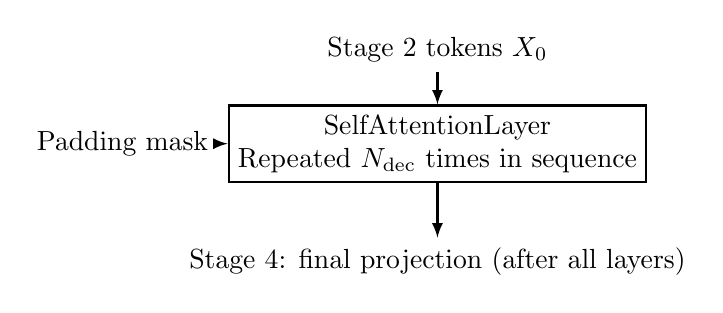
\begin{tikzpicture}[>=latex,thick]
\node (i) at (0,0) {Stage 2 tokens $X_0$};
\node[draw,align=center] (a) at (0,-1.2) {SelfAttentionLayer\\Repeated $N_{\mathrm{dec}}$ times in sequence};
\node (o) at (0,-2.7) {Stage 4: final projection (after all layers)};
\node (m) at (-4,-1.2) {Padding mask};
\draw[->] (i)--(a); \draw[->] (a)--(o);
\draw[->,dashed] (m)--(a);
\end{tikzpicture}
\end{center}

\subsection{One Encoder Layer}

The layer connections are the two residual branches shown in the earlier
layer diagram. With $x$ as the layer input, the computation is
\[
u=\mathrm{LN}_1(x),\qquad
r=x+\mathrm{SelfAttention}(u,u,u,\mathrm{mask}),
\]
\[
f=\mathrm{FFN}(\mathrm{LN}_2(r)),\qquad y=r+f.
\]
The mask enters self-attention only. Save $x$ until the first addition and
$r$ until the second. The second addition produces the layer output.
The complete review draft below expands self-attention into projections,
row-wise scores, softmax, weighted values and output projection, with a
source-compatibility masking policy and proposed sequential controller.

\section{LayerNorm: Computation and Sequential Sketch}

Both encoder normalizations use \texttt{PreNorm(D)}, which wraps
\texttt{LayerNorm(D)}. LayerNorm 1 receives the layer input and feeds
self-attention. LayerNorm 2 receives $r$ and feeds the FFN. Each preserves
$[B,L,D]$ and operates independently on the $D$ features of each token.
The two normalizations have separate learned scale and bias parameters.

For one token, compute
\[
\mu=\frac{1}{D}\sum_{i=0}^{D-1}x_i,\qquad
c_i=x_i-\mu,\qquad
v=\frac{1}{D}\sum_{i=0}^{D-1}c_i^2,
\]
\[
s=\frac{1}{\sqrt{v+\epsilon}},\qquad
z_i=c_i s,\qquad y_i=\gamma_i z_i+\beta_i.
\]
The source uses the default $\epsilon=10^{-5}$. Mean and variance are computed
from the current token during inference. The trained vectors $\gamma$ and
$\beta$, each of length $D$, are loaded from the checkpoint and shared across
tokens within this normalization instance. Variance divides by $D$.

\begin{center}
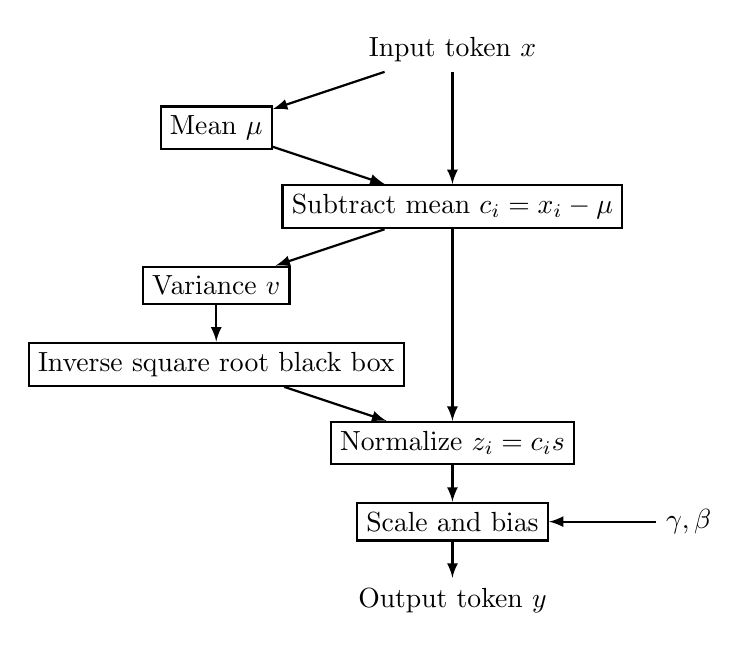
\begin{tikzpicture}[>=latex,thick,every node/.style={align=center}]
\node (x) at (0,0) {Input token $x$};
\node[draw] (m) at (-3,-1) {Mean $\mu$};
\node[draw] (c) at (0,-2) {Subtract mean\ $c_i=x_i-\mu$};
\node[draw] (v) at (-3,-3) {Variance $v$};
\node[draw] (s) at (-3,-4) {Inverse square root\ black box};
\node[draw] (n) at (0,-5) {Normalize\ $z_i=c_i s$};
\node[draw] (a) at (0,-6) {Scale and bias};
\node (p) at (3,-6) {$\gamma,\beta$};
\node (o) at (0,-7) {Output token $y$};
\draw[->] (x)--(m); \draw[->] (x)--(c); \draw[->] (m)--(c);
\draw[->] (c)--(v); \draw[->] (v)--(s); \draw[->] (s)--(n);
\draw[->] (c)--(n); \draw[->] (n)--(a); \draw[->] (p)--(a); \draw[->] (a)--(o);
\end{tikzpicture}
\end{center}

\subsection{LayerNorm FSM Proposal}

Use a token buffer, counters and reused arithmetic. The following are draft
states, not fixed cycle counts:
\begin{enumerate}
\item \textbf{IDLE}: wait for a token.
\item \textbf{LOAD AND SUM}: store $D$ features and accumulate their sum.
\item \textbf{MEAN}: calculate $\mu$.
\item \textbf{VARIANCE}: read the stored features, subtract $\mu$, square and accumulate, then divide by $D$.
\item \textbf{INV SQRT}: calculate $1/\sqrt{v+\epsilon}$ and wait for completion.
\item \textbf{NORMALIZE AND WRITE}: read features, normalize, apply $\gamma_i,\beta_i$, and write all $D$ results.
\end{enumerate}
Counter-controlled loops remain inside the active state. After the final
accepted output, return to IDLE. Multi-cycle units and memory/output stalls
must delay the corresponding transition. The complete RTL review draft below
defines the ready/valid handshake and issue/wait protocol.
The inverse-square-root implementation stays a black box.

\section{FFN: Sequential Datapath and FSM Sketch}

The FFN receives a normalized token $u$ from LayerNorm 2. Its inference path
is Linear($D,4D$), GELU, Linear($4D,D$); dropout is inactive. For each token,
\[
a_j=b_{1,j}+\sum_{i=0}^{D-1}W_{1,j,i}u_i,\qquad
h_j=\mathrm{GELU}(a_j),\qquad j=0,\ldots,4D-1,
\]
\[
f_k=b_{2,k}+\sum_{j=0}^{4D-1}W_{2,k,j}h_j,\qquad k=0,\ldots,D-1.
\]
The proposal reuses one MAC engine for both logical linear operations at
different times. Store $D$ input values. Compute each first-linear output,
apply GELU and store it. Once all $4D$ activated values are available, compute
the second linear outputs. Store or forward the $D$ results to the second
residual adder, which also receives saved $r$.

\begin{center}
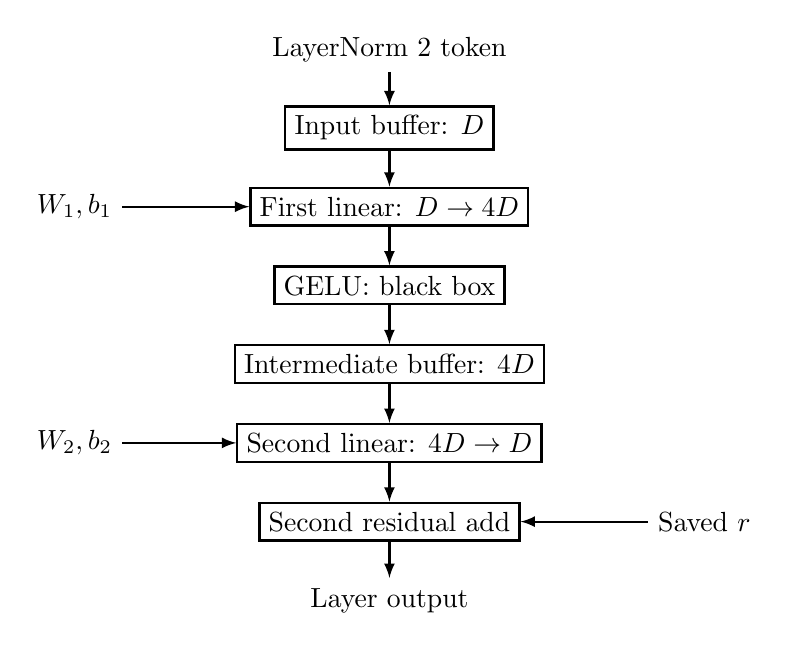
\begin{tikzpicture}[>=latex,thick,every node/.style={align=center}]
\node (i) at (0,0) {LayerNorm 2 token};
\node[draw] (b) at (0,-1) {Input buffer: $D$};
\node[draw] (l1) at (0,-2) {First linear: $D\rightarrow4D$};
\node (w1) at (-4,-2) {$W_1,b_1$};
\node[draw] (g) at (0,-3) {GELU: black box};
\node[draw] (h) at (0,-4) {Intermediate buffer: $4D$};
\node[draw] (l2) at (0,-5) {Second linear: $4D\rightarrow D$};
\node (w2) at (-4,-5) {$W_2,b_2$};
\node[draw] (a) at (0,-6) {Second residual add};
\node (r) at (4,-6) {Saved $r$};
\node (o) at (0,-7) {Layer output};
\draw[->] (i)--(b); \draw[->] (b)--(l1); \draw[->] (w1)--(l1);
\draw[->] (l1)--(g); \draw[->] (g)--(h); \draw[->] (h)--(l2);
\draw[->] (w2)--(l2); \draw[->] (l2)--(a); \draw[->] (r)--(a); \draw[->] (a)--(o);
\end{tikzpicture}
\end{center}

\subsection{FFN FSM Proposal}

\begin{enumerate}
\item \textbf{IDLE}: wait for a normalized token.
\item \textbf{LOAD INPUT}: store $D$ features.
\item \textbf{LINEAR1 INIT}: initialize the accumulator with $b_{1,j}$.
\item \textbf{LINEAR1 MAC}: accumulate $D$ products for feature $j$.
\item \textbf{GELU AND STORE}: apply GELU and store $h_j$. If another feature remains, increment $j$ and return to LINEAR1 INIT; after all $4D$ features, proceed to LINEAR2 INIT.
\item \textbf{LINEAR2 INIT}: initialize the accumulator with $b_{2,k}$.
\item \textbf{LINEAR2 MAC}: accumulate $4D$ products for output $k$.
\item \textbf{WRITE OUTPUT}: write $f_k$. If another output remains, increment $k$ and return to LINEAR2 INIT; after all $D$ outputs, finish and return to IDLE.
\end{enumerate}
The inner dot-product counters remain within the MAC states. Arithmetic
completion and memory acceptance govern progress. Each output may reach the
residual adder when its matching $r_k$ is available and the receiver is ready;
the complete token requires all $D$ outputs. No cycle count is fixed yet.

\section{Open Implementation Blocks and Status}

The encoder hierarchy, layer connections, LayerNorm arithmetic and sequential
FFN flow are now sketched. The complete RTL review draft below supplies the
remaining controller and memory contracts. Detailed implementation work includes:
\begin{itemize}
\item Self-attention: review the proposed architecture, source-compatible masking and execution schedule.
\item Inverse square root: numerical method, precision and latency.
\item GELU: approximation, supported range and latency.
\item Shared MAC: operand/accumulator widths, throughput and control interface.
\item Buffers: input/intermediate/residual storage, capacity across tokens, ports and banking.
\item Weight-memory interface: parameter layout, loading and read bandwidth.
\end{itemize}
Precision, reset, handshake, stalls and top-level scheduling have proposed
definitions in the complete RTL review draft below. These supersede the earlier
high-level FSM sketches where more detail is supplied. Final projection and
aggregation also have draft controllers. Numerical calibration, RTL implementation
and supervisor approval remain separate milestones.

\section{Self-Attention: Connected Sequential Datapath}

All normalized tokens enter the Q, K and V projections, each with its own
weights and biases. The proposal stores all projected tokens, computes one
head/query score row, applies the source-compatible mask and softmax, and
multiplies that probability row by stored V. Head outputs are written into
the joined Z layout before the final D-to-D output projection.
The V path bypasses score generation and softmax. The following section
specifies counters, source-mask semantics, controller transitions and memories.

\begin{center}
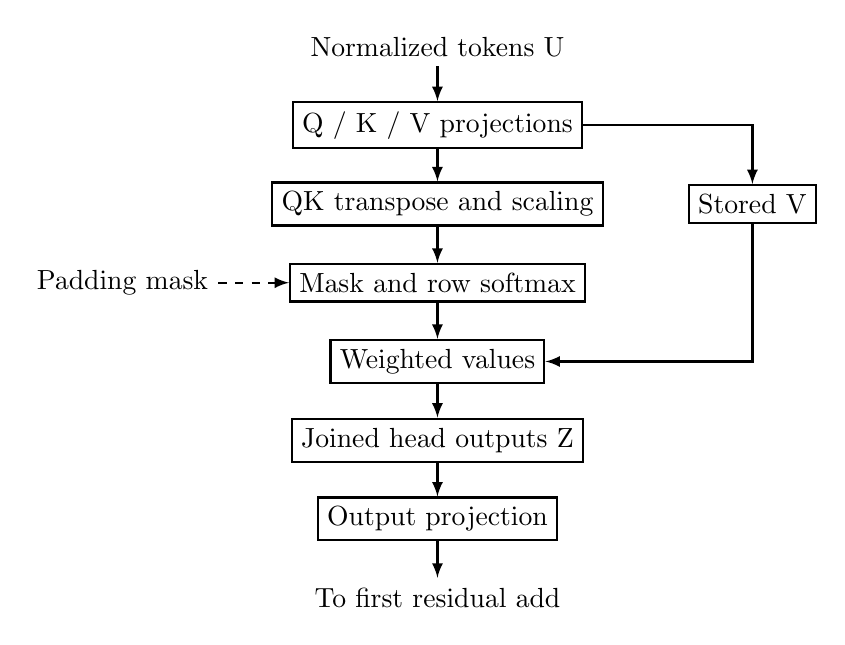
\begin{tikzpicture}[>=latex,thick,every node/.style={align=center}]
\node (i) at (0,0) {Normalized tokens U};
\node[draw] (q) at (0,-1) {Q / K / V projections};
\node[draw] (s) at (0,-2) {QK transpose and scaling};
\node[draw] (a) at (0,-3) {Mask and row softmax};
\node (m) at (-4,-3) {Padding mask};
\node[draw] (v) at (4,-2) {Stored V};
\node[draw] (w) at (0,-4) {Weighted values};
\node[draw] (z) at (0,-5) {Joined head outputs Z};
\node[draw] (p) at (0,-6) {Output projection};
\node (o) at (0,-7) {To first residual add};
\draw[->] (i)--(q); \draw[->] (q)--(s); \draw[->] (q)-|(v);
\draw[->] (s)--(a); \draw[->,dashed] (m)--(a); \draw[->] (a)--(w);
\draw[->] (v)|-(w); \draw[->] (w)--(z); \draw[->] (z)--(p); \draw[->] (p)--(o);
\end{tikzpicture}
\end{center}

% BEGIN REVIEWED MATHEMATICS
\section{Reviewed Architecture: Mathematics and Execution Schedule}
This section consolidates the joint review of 25 September 2026. The sequential schedule is the working baseline; numerical formats, nonlinear implementations, memory macros and timing remain provisional. It is not a claim of completed RTL or supervisor approval. Equations below describe real arithmetic; every stored hardware value follows the explicitly selected quantization contract.

\subsection{Dimensions, parameters and frame ownership}
One frame is active: $B=1$. Host batches are submitted sequentially. There are $M$ read slots, $N$ positions per read, $L=MN$ tokens, flattened input width $F$, feature width $D$, $H$ heads, head width $d=D/H$, and $K=N_{dec}$ layers. Require $D$ divisible by $H$. These dimensions come from the configuration matching the checkpoint; they are not learned. Weights, biases, position/read embeddings and normalization affine parameters are learned and persist between frames.
\[
t=mN+n,\qquad 0\leq m<M,\quad 0\leq n<N,\quad 0\leq j<D.
\]
Addresses and loop counters are exact unsigned integers, not quantized activations. Use terminal comparisons and explicit resets, not accidental binary overflow. A counter advances only after the corresponding accepted transaction or committed result.
The frame controller loads features and mask, runs embedding, position additions, encoder, final projection and aggregation, then transfers $N$ output logits. Stored outputs are ready before transfer; successful frame completion requires all $N$ output handshakes. Requests remain stable while stalled, and completion remains asserted until accepted. Invalid descriptors or arithmetic faults follow the error path rather than normal completion.

\subsection{Shared dot and linear engines}
For input length $I$ and output length $O$, the mathematical linear operation is
\[
y_j=b_j+\sum_{r=0}^{I-1}W_{j,r}x_r,\qquad 0\leq j<O.
\]
\begin{itemize}
\item Dot INIT\_ACC: initialize a widened accumulator to aligned bias or zero; set $r=0$.
\item READ\_INPUT\_REQ/WAIT and READ\_WEIGHT\_REQ/WAIT: capture both operands. Operand B can be a learned weight, key or value; it is not always a weight.
\item ISSUE\_MAC/WAIT\_MAC: compute $A\leftarrow A+a_rb_r$ once, capture completion, then NEXT\_TERM increments $r$ or enters DONE. DONE returns the widened result without destination narrowing.
\item Linear READ\_BIAS, DOT\_COMMAND/WAIT: select the output row and run its dot product. ROUND\_SATURATE converts once to the destination format. WRITE\_REQ/WAIT commits the result; NEXT\_OUTPUT advances $j$ or completes.
\end{itemize}
The source vector must survive all $O$ dot products. Logical projections reuse this engine sequentially; diagram branches do not imply parallel multipliers. Memory adapters and scalar engines have request/wait substates, so a named arithmetic state is not necessarily one clock cycle.

\subsection{Layer normalization: common engine for F or D features}
For a vector $x$ of length $J$, with separately loaded affine parameters,
\[
\mu=\frac{1}{J}\sum_{j=0}^{J-1}x_j,\qquad
v=\frac{1}{J}\sum_{j=0}^{J-1}(x_j-\mu)^2,\qquad
g=(v+\epsilon)^{-1/2},\qquad
y_j=\gamma_j(x_j-\mu)g+\beta_j.
\]
Use the population variance (denominator $J$, not $J-1$). The reference default epsilon is $10^{-5}$. Gamma and beta are learned; mean and variance are computed for every current token.
\begin{itemize}
\item LOAD\_AND\_SUM: retain the input vector and accumulate its sum in widened storage.
\item MEAN: multiply by the configured reciprocal $1/J$; preserve the selected precision.
\item VARIANCE: reset the feature counter and sum centered squared differences in widened storage, then scale by $1/J$.
\item INV\_SQRT: add epsilon in a format that represents it, issue the scalar operation and wait for its result.
\item NORMALIZE\_WRITE: reset the counter; subtract mean, multiply by $g$ and gamma, add beta, convert and commit each output. DONE follows the final write.
\end{itemize}
The centered two-pass calculation is the proposed baseline. Its operation order can differ from a floating-point library kernel. Epsilon must not disappear through quantization. Variance, inverse square root and affine scaling are high-risk numerical areas.

\subsection{Stage 1: input embedding}
For each flattened token $x_t\in\mathbb{R}^{F}$,
\[
u_t=\operatorname{LN}_{F}(x_t),\qquad
v_{t,j}=b^{emb}_j+\sum_{r=0}^{F-1}W^{emb}_{j,r}u_{t,r},\qquad
e_t=\operatorname{LN}_{D}(v_t).
\]
LOAD\_TOKEN captures $F$ values; LN\_F runs the common normalization engine; LINEAR\_F\_TO\_D runs $D$ dots of length $F$; LN\_D uses its own affine parameters; WRITE\_TOKEN commits $D$ outputs. NEXT\_TOKEN repeats until $L$ tokens are stored. Do not skip padded tokens or overwrite the linear input scratch before all output features complete.

\subsection{Stage 2: trained position and read embeddings}
\[
a_{m,n,j}=e_{mN+n,j}+P_{n,j},\qquad
X^{(0)}_{mN+n,j}=a_{m,n,j}+E_{m,j}.
\]
P and E are loaded trained tables, not values regenerated during inference. INIT sets $(m,n,j)=(0,0,0)$; READ\_X, READ\_P, ADD\_P, READ\_E, ADD\_E and WRITE perform the two additions with separate destination conversions. With equal fractional scales, conversion need not discard fractional bits but can still saturate.
After each committed write, increment $j$ unless $j=D-1$; then reset $j$ and advance $n$. At $n=N-1$, reset $n$ and advance $m$. Finish at the last feature of read $M-1$. No runtime modulo or division is required. The padding mask bypasses this arithmetic unchanged.

\subsection{Stage 3: one physical layer repeated K times}
For layer $k$, with its own learned parameters,
\[
U=\operatorname{LN}_{1,k}(X^{(k)}),\qquad O=\operatorname{Attn}_{k}(U),\qquad R=X^{(k)}+O,
\]
\[
T=\operatorname{LN}_{2,k}(R),\qquad G=\operatorname{FFN}_{k}(T),\qquad X^{(k+1)}=R+G.
\]
Schedule LN1\_ALL\_TOKENS, ATTENTION, RESIDUAL1\_ALL, then LN2\_TOKEN, FFN\_TOKEN and RESIDUAL2\_TOKEN for each token. Preserve original X through attention and preserve R through its FFN. In-place residual writes are safe only after both operands are captured. Layer completion follows the last residual-2 write. The encoder then selects the next layer's parameter bases, or releases $X^{(K)}$ to Stage 4. Dropout is disabled in inference.

\subsection{Attention projections, head slices and score rows}
\[
Q_{t,j}=b^Q_j+\sum_{r=0}^{D-1}W^Q_{j,r}U_{t,r},\quad
K_{t,j}=b^K_j+\sum_{r=0}^{D-1}W^K_{j,r}U_{t,r},\quad
V_{t,j}=b^V_j+\sum_{r=0}^{D-1}W^V_{j,r}U_{t,r}.
\]
Here K as a tensor means keys; the layer count is identified by context as $N_{dec}$. The outer QKV controller selects projection and token; linear selects output feature; dot selects input term. Finish all Q tokens, then all K tokens, then all V tokens. Each projection uses all $D$ input features, not just one head slice.
\[
s_{a,i,j}=\frac{1}{\sqrt d}\sum_{r=0}^{d-1}Q_{i,ad+r}K_{j,ad+r}.
\]
For fixed head $a$ and query $i$, INIT\_KEY sets $j=0$. ISSUE\_DOT/WAIT\_DOT uses length $d$, zero initial sum, bases $Q_{base}+iD+ad$ and $K_{base}+jD+ad$, and stride one. ISSUE\_SCALE/WAIT\_SCALE multiplies by a precomputed $1/\sqrt d$; WRITE\_SCORE converts and commits. NEXT\_KEY repeats for $L$ keys. Only one score row is stored, not an $L$ by $L$ matrix.

\subsection{Mask and softmax}
For a non-padded query row,
\[
m_s=\max_j s_j,\qquad e_j=\exp(s_j-m_s),\qquad
S_{exp}=\sum_{j=0}^{L-1}e_j,\qquad p_j=e_j/S_{exp}.
\]
CHECK\_MASK chooses the normal path or the uniform bypass. FIND\_MAX initializes from the first score, not zero. EXP\_AND\_SUM resets the counter, stores each exponential and accumulates $S_{exp}$. RECIPROCAL requests $1/S_{exp}$ once. PREPARE\_VALUE and WRITE\_PROBABILITY multiply each saved exponential by that reciprocal, convert and commit; NEXT\_ENTRY repeats until the row is ready.
The source padding shape is $[B,1,L,1]$: it masks query rows, not key columns. A padded query has all scores replaced by the same finite sentinel, yielding $p_j=1/L$ in real arithmetic. The hardware bypass uses a stored quantized $1/L$ and the same probability writer. Valid queries still attend to padded keys. This behavior must not be silently corrected. Optional static masking is outside the baseline until agreed. Quantized probabilities need not sum exactly to one; test the discrepancy. A nonpositive exponential sum raises an error.

\subsection{Weighted values and output projection}
\[
Z_{i,ad+r}=\sum_{j=0}^{L-1}p_j V_{j,ad+r},\qquad
O_{i,j}=b^O_j+\sum_{r=0}^{D-1}W^O_{j,r}Z_{i,r}.
\]
Weighted INIT\_FEATURE sets $r=0$. ISSUE\_DOT/WAIT\_DOT uses length $L$, probability stride one, V stride $D$, zero initial sum and unsigned-probability times signed-value arithmetic. ROUND\_SATURATE and WRITE\_RESULT commit directly to $Z_{base}+iD+ad+r$. NEXT\_FEATURE repeats for $d$ features while preserving the probability row. Only then advance query, and after the last query advance head. Joined heads need no separate copy operation.
Once every head/query result is stored, output projection issues one shared linear(D,D) command per token, waits for its writes, then advances the token. This mixes all heads. Its completion releases O to the first residual addition with original X, not normalized U.

\subsection{FFN and residual additions}
For the LN2 output token $T_t$,
\[
h_j=b^1_j+\sum_{r=0}^{D-1}W^1_{j,r}T_{t,r},\quad 0\leq j<4D,
\]
\[
g_j=\operatorname{GELU}(h_j)=\frac{h_j}{2}\left(1+\operatorname{erf}\left(\frac{h_j}{\sqrt 2}\right)\right),\qquad
G_{t,j}=b^2_j+\sum_{r=0}^{4D-1}W^2_{j,r}g_r.
\]
LINEAR1 runs D-to-4D with bias. GELU requests and writes every hidden feature; retain all $4D$ activated values before LINEAR2 runs 4D-to-D with bias. There is no second GELU. The exact-erf formula is the reference target, not a promise of a hardware erf implementation.
Both residual controllers capture left and right values, align their scales, add in a widened format, convert and commit. Their equations are $R_{t,j}=X_{t,j}+O_{t,j}$ and $X^{next}_{t,j}=R_{t,j}+G_{t,j}$. Feature counters advance after write completion. Residual 2 completes the current token before the layer advances.

\subsection{Stage 4: final projection and aggregation}
\[
z_t=b^{final}+\sum_{j=0}^{D-1}w^{final}_j X^{(K)}_{t,j}.
\]
INIT\_TOKEN, ISSUE\_LINEAR, WAIT\_LINEAR and NEXT\_TOKEN run D-to-1 for all $L$ tokens. The linear controller owns the logit write: there is no second STORE\_LOGIT state. The binary target uses one unrestricted logit, not a probability or a percentage.
Let $p^{mask}_{m,n}=1$ denote padding. For $M>1$ the source aggregation is
\[
c_m=\begin{cases}1&\text{if every }p^{mask}_{m,n}=0,\\0&\text{otherwise},\end{cases}
\quad C=\sum_m c_m,\quad S_n=\sum_m(1-p^{mask}_{m,n})z_{mN+n},\quad y_n=S_n/C.
\]
COUNT\_VALID\_SLOTS and CHECK\_COUNT precede one RECIPROCAL request for $1/C$ per frame. For each position, SUM\_READS accumulates the masked numerator; SCALE multiplies by the saved reciprocal; WRITE commits $y_n$; NEXT\_POSITION repeats. Partially padded reads can contribute to the numerator without contributing to C: preserve this nonstandard source rule and confirm permitted inputs. For $C=0$, hardware reports an error, an explicit guard beyond the source's nonfinite arithmetic.
For $M=1$, copy $y_n=z_n$ directly, without masking or averaging, matching the source branch. Optional hard decisions are $\hat b_n=1$ when $y_n>0$ and zero otherwise. If a probability is needed externally, $\sigma(y_n)=1/(1+\exp(-y_n))$; sigmoid is unnecessary for the zero-threshold decision and is not added to the core.

\subsection{Numerical observations and remaining implementation boundaries}
Record the floating-point reference, widened fixed-point intermediate and stored fixed-point value separately. The widened value may already include upstream quantization error. Capture indices, formats, rounding-change, saturation and overflow flags once per accepted conversion event, not repeatedly during stalls. Simulation observation needs no additional compute FSM state. Optional on-chip snapshots require a separately bounded buffer and readout design; no compute stall or wide-result bypass is assumed.
The remaining arithmetic black boxes are GELU, exponential, reciprocal and inverse square root, including their reduction/scaling precision. Their request/response boundaries and schedule are specified; their arithmetic implementation is not frozen. Accumulator widths, memory mapping, clock target and resource feasibility require measurement and synthesis. Earlier numeric contracts are experimental candidates, not demonstrated accuracy or latency guarantees.

% END REVIEWED MATHEMATICS

% BEGIN GENERATED RTL REVIEW
\section{RTL Specification: Complete Review Draft}

Review baseline consolidated: 25 September 2026. Sequential schedules are reviewed working choices; numerical contracts and physical feasibility remain provisional. This is not a claim of completed RTL or supervisor approval.
Status: proposed architecture for Amit's review, not implemented or numerically validated RTL.

\subsection{Scope and evidence}

Inputs are prepared window features and a padding mask. Outputs are binary logits. Window generation, training, hard decisions and outer decoding are outside the core. All five software stages are included. Dropout is disabled for inference.

Source: BCJRFormer/bcjrformer/models/bcjrformer.py, especially constructor and forward; BCJRFormer/bcjrformer/models/modules.py, especially MultiHeadedAttention, FeedForward, SelfAttentionLayer and TransformerEncoder. The example model YAML has D=16, H=2, N\_dec=1 and M=1. It does not prove the configuration of a trained checkpoint.

\subsection{Proposed configuration}

One frame at a time, B=1. Compile-time parameters: N encoded positions, M read slots, F window features, D model width, H heads, K encoder layers; L=M*N and d=D/H. Require all dimensions positive and D divisible by H. Preserve the general M>1 path even if the first test uses M=1. N and F must be selected with the dataset/checkpoint, not guessed from the model YAML.

Use sequential arithmetic and one exclusive shared dot-product engine. Keep all Q/K/V vectors for a layer, but only one attention score row. Do not parallelize layers or frames in this baseline. The same encoder hardware iterates over layers with different parameter bases.

Numerical proposal, pending calibration: signed 16-bit stored activations and weights with 10 fractional bits (range -32 to 31.9990234375). Standard linear and QK dot products use a signed 48-bit accumulator with 20 fractional bits. Products are exact 32-bit signed values before extension. Biases are stored at 16/10 and shifted left by 10 before accumulator initialization. The same physical engine also supports a 24-bit unsigned probability times a 16-bit signed value; zero-extend probabilities before multiplication and use a signed 64-bit accumulator with 32 fractional bits for weighted values. Set the physical accumulator width to 64 and sign-extend the standard 48-bit mode while checking its declared range. Round to nearest, ties to even, then saturate on narrowing. Record saturation and accumulator-overflow flags. This format is a starting experiment, not an accuracy claim. Wider formats and per-tensor scales may be needed.

LayerNorm means use signed 32-bit/20-fraction values. Centered differences use signed 40-bit/20-fraction values, with 80-bit full products and 96-bit/40-fraction variance accumulation before division by V. Variance plus epsilon is unsigned 48-bit/32-fraction at the rsqrt interface. Represent softmax exponentials and probabilities in unsigned 24-bit/22-fraction format, with a 64-bit/22-fraction sum. Score rows use signed 48-bit/20-fraction values, retaining QK precision through scaling (not 16-bit narrowing). All reductions check overflow. Compile-time bounds: V<=65535, L<=65535, and d<=65535; reject larger configurations. These are proposed numeric bounds, not practical SRAM capacity targets. Precision adapters are explicit operations; epsilon is round(1e-5 * 2\textasciicircum{}32)/2\textasciicircum{}32 and must not round to zero. Implementing the wide scalar path serially is allowed; it is distinct from the shared matrix dot engine. Accuracy must be established by bit-accurate tests before RTL is frozen.

\subsection{Common transaction protocol}

\subsection{Scalar arithmetic and constants}

For the proposed bit-accurate baseline, constants are elaboration-time values rounded to nearest, ties to even: 1/F and 1/D use unsigned40/32; 1/sqrt(d) uses unsigned32/30; the uniform attention probability 1/L uses unsigned24/22. They are not learned weights. Runtime 1/C uses the reciprocal unit after checking C>0.

LayerNorm sum is signed48/10. Multiply by unsigned40/32 (zero-extended for signed arithmetic), retaining a signed89/42 product, then round to signed32/20 mean. Center by extending the input to signed40/20. Accumulate full centered squares in unsigned96/40; multiply the variance sum by unsigned40/32 using a full unsigned136/72 intermediate, then round to unsigned48/32 and add epsilon. Such wide intermediate registers may be implemented by a serial scalar datapath; they do not travel through the 96-bit memory adapter. Multiply centered signed40/20 by zero-extended rsqrt unsigned32/20 to signed73/40; round to signed32/20 normalized value. Multiply by signed16/10 gamma to signed48/30, add beta extended to signed49/30, then round/saturate to signed16/10. All intermediate range violations raise numerical error rather than silently wrapping.

Scale signed48/20 QK scores by unsigned32/30 using signed81/50 full multiplication, then round to signed48/20. Subtract the row maximum in signed49/20; compare with -16 before narrowing the retained exp input to signed48/20. Normalize unsigned24/22 exponentials with unsigned40/32 reciprocal through unsigned64/54, then round to unsigned24/22. Independent probability rounding need not sum exactly to one; measure that error in verification. Aggregate unmasked logits using signed48/10 sum; multiply by runtime unsigned40/32 reciprocal into signed89/42, then round/saturate to signed16/10. Position and residual additions use signed17/10 before narrowing. The final logit storage proposal is signed16/10. These are explicit draft rounding points, not proof of equivalence to floating-point inference.

All modules use clk and synchronous active-high rst. On reset: deassert output valid, clear busy/counters/ownership and invalidate configuration/frame state. Memory contents need not clear because valid flags prevent reads of stale data.

Commands use cmd\_valid/cmd\_ready. Capture descriptors only when both are high. Only one command is outstanding per engine. Results use rsp\_valid/rsp\_ready with rsp\_error; hold response and error stable until accepted. A response indicates all commanded writes have committed, not merely that arithmetic has started. Address/data requests and responses each use ready/valid. Counters advance on accepted work or completed results, never on an unaccepted request. If stalled, hold payload/address/control stable. No timeout is inferred; a diagnostic watchdog is optional and outside the baseline behavior.

Arithmetic primitives use req\_valid/req\_ready, operands and operation tag, followed by rsp\_valid/rsp\_ready, result and error. Latency may vary; controllers wait for the response. One outstanding request avoids tag-reordering logic. Errors latch at top level, stop new requests, drain any accepted transaction, and produce one error completion. Reset is required before retry after an error in this initial proposal.

\subsection{Top-level ports and load order}

bcjrformer\_core: clk, rst; parameter-write channel \{valid,ready,addr,data\}; parameter\_commit; frame command \{valid,ready\}; feature input \{valid,ready,data,last\}; mask input \{valid,ready,bit,last\}; logit output \{valid,ready,data,index,last\}; completion \{valid,ready,error\}; busy; numerical-status flags.

Parameter writes are accepted only in IDLE before a frame, sequentially from address zero, with the exact manifest length. Reject out-of-order, duplicate and out-of-range addresses. parameter\_commit is accepted only after all expected words have committed; any new load invalidates the old image. Host supplies the matching configuration manifest; a checksum is a verification/host responsibility. No run-time dimension changes.

parameter\_commit is a one-cycle strobe legal only while IDLE after the last parameter write response; it has no ready signal. An illegal strobe latches a protocol error and requires reset. Frame-command ready is high only for a committed image with no outstanding parameter transaction and no parameter write/commit presented that cycle. Parameter writes take priority over frame commands. Top-level data widths are 16 for weights/features/logits, one for mask/last/valid/ready/error/busy, PARAM\_ADDR\_W for parameter address, and max(1,ceil(log2(N))) for output index. Feature and mask counters are sized from their complete bank lengths, not the 16-bit vector descriptor count. Status bits distinguish saturation (sticky, nonfatal), arithmetic overflow/domain error, and protocol error (fatal). Saturation clears at each accepted frame; fatal status clears only on reset.

After frame command acceptance: load L*F features in m,n,f order, then L mask bits in m,n order. Check last exactly at the specified final element. Early or missing last is a frame error. No feature/mask overlap is required. Compute starts after both loads. Output N logits in n order with last on n=N-1. Completion is asserted after the final output transfer; output backpressure must not discard or duplicate logits.

\subsection{Module hierarchy and contracts}

\begin{itemize}
\item Module -- Inputs / read ownership -- Outputs / completion
\item core\_ctrl -- Complete frame and parameter image -- Commands the five stages and emits logits
\item embedding\_ctrl -- Features [L,F]; three normalization/linear parameter sets -- Stage 1 X [L,D]
\item position\_ctrl -- X, P[N,D], E[M,D] -- In-place X+P+E [L,D]
\item encoder\_ctrl -- X and mask; layer parameter base -- K layers completed, X [L,D]
\item layer\_ctrl -- One layer input X [L,D] -- Updated layer output [L,D]
\item layernorm\_ctrl -- Vector length V (F or D), source/destination addresses, gamma/beta bases -- One V-element normalized vector
\item linear\_ctrl -- Input length I, output length O, vector/weight/bias/output bases -- O outputs, bias included
\item attention\_ctrl -- All normalized tokens U [L,D], padding mask, optional static mask -- O [L,D] after output projection
\item softmax\_ctrl -- One L-element score row plus mask tags -- One L-element probability row
\item ffn\_ctrl -- One normalized token [D], FFN parameters -- One FFN token [D]
\item residual\_ctrl -- Two D-element vectors, destination -- D committed sums
\item final\_ctrl -- Encoder tokens [L,D], final weights/bias -- Per-read logits [L]
\item aggregation\_ctrl -- Logits [M,N] and original mask [M,N] -- N logits and denominator status
\item dot\_engine -- I, operand-memory descriptors, accumulator initial value -- One widened dot product
\item parameter\_mem -- Read address or idle-time host write -- Parameter data / accepted write
\item scratch\_mem -- Exclusive owner requests -- Read/write completion
\item exp\_unit, reciprocal\_unit, rsqrt\_unit, gelu\_unit -- Numeric requests under the common protocol -- Numeric result/error with bounded input domain
\end{itemize}


Address widths are max(1,ceil(log2(depth))) for each bank. Counter widths must represent the terminating count (ceil(log2(count+1))), or use last-index comparisons without overflow. Parameter arithmetic uses elaboration-time constants and checks total address range.

Descriptor register contracts: layernorm=\{V,src,dst,gamma\_base,beta\_base\}; linear=\{I,O,src,dst,W\_base,b\_base\}; residual=\{V,left,right,dst\}; attention=\{L,D,H,U\_base,O\_base,Q\_base,K\_base,V\_base,Z\_base,layer\_param\_base\}; dot=\{I,A\_base,A\_stride,B\_base,B\_stride,mode,acc\_init\}; softmax=\{L,score\_base,prob\_base,padded\_query\}. Counts are 16-bit unsigned under the declared bounds; every descriptor count, including FFN length 4D and layer count K, must fit 1..65535. Bases and strides are BANK\_ADDR\_W unsigned; products of dimensions and all memory-size calculations use at least 64-bit elaboration/host arithmetic and must fit their bank. Descriptors are latched on command acceptance and immutable until completion. mode selects signed16xsigned16/20-fraction or unsigned24xsigned16/32-fraction accumulation. acc\_init is signed64 in the selected binary point.

Memory requests carry valid, ready, write, bank, address, data and format; write responses acknowledge commitment and read responses carry data. Native banks use their declared width; the common adapter payload is 96 bits with unused upper bits zero on writes and canonical sign/zero extension on reads. Bank/format mismatches raise errors. Parameter words remain 16 bits except static-mask bits and the host-independent wider constants. No byte enables or burst ordering are required for the draft.

\subsection{Memory ownership and lifetime}

\begin{itemize}
\item Storage -- Elements -- Lifetime / owner
\item --- -- ---: -- ---
\item Feature memory -- L*F -- Load through completion of embedding
\item Padding bits -- L -- Whole frame; immutable during compute
\item X residual bank -- L*D -- Holds original layer input until attention residual addition; then holds r until FFN residual addition
\item U normalized bank -- L*D -- LayerNorm 1 output until Q/K/V creation completes
\item Q, K, V banks -- 3*L*D -- One complete attention layer
\item Z bank -- L*D -- Concatenated weighted-head outputs until output projection completes
\item Attention output bank -- L*D -- Output projection until residual addition
\item Token scratch -- max(F,D) -- Normalization or FFN input, exclusive sequential use
\item FFN hidden -- 4D -- One token's GELU outputs until second linear completes
\item Vector result scratch -- max(D,4D) -- Linear/normalization result, assigned exclusively
\item Score, exponential, probability rows -- 3L -- One head/query row; each has its own numeric format
\item Logits -- L -- Final projection through aggregation
\item Aggregated output -- N -- Aggregation through host transfer
\end{itemize}


Add scalar scratch registers for mean, centered difference, squared value, variance, row maximum, widened row sum, reciprocal and loop indices. Optional static-mask storage contains L*L bits and is immutable during a frame. All listed banks are logically separate in this conservative draft; capacity reduction through aliasing requires a later lifetime proof.

Stage 1 uses token scratch for F-element input normalization in place: both statistics passes finish before any output overwrites its corresponding input. The F-to-D projection writes separate vector result scratch, followed by in-place D-element normalization there, then copies D results to X. FFN input scratch and hidden/result banks remain separate while needed. No linear command may alias its source and destination when future outputs still need the original source vector.

Proposed single-port synchronous banks, abstracted behind request/response adapters. Dot engine reads operand A, captures it, then operand B, captures it, then issues MAC and waits. It does not assume two reads per cycle. Banks may later be dual-ported without changing controller contracts. No other controller uses shared arithmetic or scratch while an owner command is outstanding.

Residual writes are in-place only after both operands at that address have been captured. All Q/K/V must exist before attention score evaluation. All head results for a token must exist before its output projection. All attention outputs are computed before overwriting X with first residual sums. FFN is then processed token by token; each r token survives until its own second residual addition commits.

Parameter tensors use software Linear layout W[out,in], row-major: base+out*I+in. Token address=t*D+i; t=m*N+n. Head component address=t*D+a*d+r. P address=n*D+i, E address=m*D+i. Layer parameters have distinct base addresses. A generated parameter manifest must list all tensor bases, shapes, formats and checksums. Parameter count in 16-bit words is 2F + DF + 3D + ND + MD + K*(12D\textasciicircum{}2+13D) + D+1: Stage 1 has two LayerNorms and an F-to-D linear; each encoder layer has four D-to-D projections, two FFN projections, and two LayerNorms; the final projection has D weights and one bias. Optional mask bits and numeric constants are separate. Sum bank sizes using their individual widths to obtain bit capacity once F,N,M,D,H,K are selected.

\subsection{FSM conventions}

Every ISSUE state waits for request acceptance, every WAIT state waits for accepted completion, and every WRITE waits for memory acceptance/completion. The compact sequences below expand to those states where needed. No transition proceeds on busy alone. All terminal states hold response until accepted. Primitive errors take the error path described above.

On accepted command, clear the command's loop indices and reduction registers; latch immutable lengths and bases. Each nested-loop restart clears its inner index and accumulator before issuing work. Linear output accumulators initialize from the current bias, never the previous output. LayerNorm sum and variance sum clear separately before their passes; softmax maximum initializes from the first score (not zero), and exp sum clears before its pass. Aggregation clears C at frame start, a slot-valid flag at each new slot (initialized true), and the numerator at each new position. The slot-valid flag ANDs the inverse mask bit for all N positions before contributing to C. Capture a memory or primitive result only on its response handshake; advance the associated index only once that operation's dependent write, if any, commits.

For attention, inner score-key index j resets for each (head a, query i); dot term index resets for each key. Weighted-value component r resets for each query; its dot term runs over j. On query completion: if i+1<L, increment i; else set i=0 and, if a+1<H, increment a; otherwise proceed to output projection. Output-token index restarts at zero. For the layer FFN loop, t restarts at zero after the first residual pass; for each next layer, all token/head/feature indices restart and only the parameter base advances. Every compact terminal DONE returns to command-ready IDLE only after response acceptance.

\subsection{Frame and encoder control}

Core: IDLE -> LOAD\_FEATURES -> LOAD\_MASK -> EMBED -> POSITION -> ENCODER -> FINAL -> AGGREGATE -> OUTPUT -> COMPLETE -> IDLE. Each compute state launches once and waits. Feature/mask/output counters increment only on transfer. Bad packet counts or uncommitted parameters prevent compute.

Encoder: INIT\_LAYER(k=0) -> RUN\_LAYER -> WAIT\_LAYER -> NEXT\_LAYER. If k+1<K increment layer index and parameter base, otherwise DONE. One physical layer datapath is reused.

Layer: LN1\_ALL\_TOKENS -> ATTENTION -> RESIDUAL1\_ALL -> LN2\_TOKEN -> FFN\_TOKEN -> RESIDUAL2\_TOKEN -> NEXT\_TOKEN -> DONE. LN2/FFN/residual2 loop t=0..L-1. The mask is supplied only to attention; normalization/FFN do not skip padded tokens in compatibility mode.

\subsection{Shared linear and dot engines}

Linear: INIT\_OUTPUT(j=0) -> READ\_BIAS -> DOT\_COMMAND -> DOT\_WAIT -> ROUND\_SATURATE -> WRITE -> NEXT\_OUTPUT. Repeat for j<O; complete after O committed writes. Dot: INIT\_ACC -> READ\_A -> READ\_B -> MAC\_ISSUE -> MAC\_WAIT -> NEXT\_TERM. Repeat i<I; return widened accumulator after the final term. This fixes sequential ordering without assuming a particular MAC latency.

\subsection{Stage 1 input embedding}

For t=0..L-1: LOAD\_TOKEN -> LN\_F -> LINEAR\_F\_TO\_D -> LN\_D -> WRITE\_TOKEN -> NEXT\_TOKEN. Each subcommand completes before its scratch is reused. First and second normalization parameters are separate, and both are separate from encoder normalization parameters.

\subsection{Stage 2 position and sequence embedding}

INIT(m=0,n=0,j=0) -> READ\_X -> READ\_P -> ADD\_P -> READ\_E -> ADD\_E -> WRITE -> NEXT\_INDEX -> DONE. Mathematical token mapping t=m*N+n; hardware uses exact integer nested counters, not runtime modulo/division. After a committed write, increment j; at j=D-1 reset j and advance n; at n=N-1 reset n and advance m; finish after m=M-1. Preserve separate conversion points after each add. P/E are loaded trained values, not generated positional sinusoids.

\subsection{LayerNorm}

LOAD\_AND\_SUM -> MEAN -> VARIANCE -> RSQRT -> NORMALIZE\_AND\_WRITE -> DONE. LOAD\_AND\_SUM stores V values and uses widened sum. MEAN applies 1/V. VARIANCE rereads every x\_i, forms x\_i-mu, squares and sums, then divides by V. RSQRT requests 1/sqrt(v+epsilon) once. NORMALIZE\_AND\_WRITE rereads x\_i, subtracts mu, multiplies by reciprocal standard deviation and gamma\_i, adds beta\_i, narrows and writes. Each loop increments after its corresponding accepted operation; the inverse-square-root response must arrive before normalization starts. Stats/squares use a specified widened format in the eventual bit-accurate model.

\subsection{Self-attention}

PROJ\_Q\_ALL -> PROJ\_K\_ALL -> PROJ\_V\_ALL -> INIT\_HEAD\_QUERY -> SCORE\_ROW -> SOFTMAX\_ROW -> WEIGHTED\_VALUES -> NEXT\_QUERY\_HEAD -> OUTPUT\_PROJECTION -> DONE.

Q/K/V each run L linear(D,D) commands with distinct parameters and bias. For head a and query i, SCORE\_ROW loops key j=0..L-1, accumulates sum\_r Q[i,a,r]*K[j,a,r] for r<d, scales by 1/sqrt(d), records mask tags and writes score[j]. After softmax returns, WEIGHTED\_VALUES loops r<d and accumulates sum\_j probability[j]*V[j,a,r], writing Z[i,a*d+r]. Increment query i; wrap at L and increment head a; after H heads run linear(D,D) with output-projection weights/bias for every token. Head splitting and joining are address mappings, not extra multipliers.

\subsection{Mask semantics: source compatibility must be explicit}

The expanded controller definitions in the joint-review section below refine the compact schedules above. They record the working architecture agreed with Taimor, not supervisor approval or numerical sign-off.

The current source reshapes padding\_mask to [B,1,L,1], which masks QUERY ROWS, not key columns. It fills masked scores with finite -1e9, then applies softmax. A fully filled row is uniform in the floating-point reference. Do not silently implement key masking or zero rows while claiming source equivalence.

Proposed default is SOURCE\_COMPAT mode with no static mask, matching the inspected marker-model path pending confirmation of its selected configuration. For a padded query, directly set its probability row to 1/L; do not represent -1e9 in the narrow fixed-point format. Valid queries retain all keys, including padded keys. Optional static mask support requires separate L*L mask storage and a declared layout; exclude it from the baseline only if Amit approves the no-static-mask configuration. If static mask support is enabled, retain symbolic sentinel tags, handle fully masked rows as uniform, and validate the finite-sentinel approximation against reference scores. A KEY\_MASKED mode is a different algorithm requiring explicit approval and independent reference results.

\subsection{Softmax}

READ\_ROW\_MAX -> EXP\_AND\_SUM -> RECIPROCAL -> NORMALIZE\_ROW -> DONE. Reduce over j, subtract row maximum, issue exp for each score difference, store each result and accumulate widened positive sum. Request reciprocal once; multiply each saved exponential by it and write probability[j]. A full sentinel row takes the uniform-row path. A nonpositive sum or invalid primitive result raises error. Clipping range and approximation errors are numerical decisions awaiting calibration.

\subsection{FFN}

LOAD\_INPUT -> LINEAR1\_INIT -> LINEAR1\_MAC -> GELU\_AND\_STORE -> LINEAR2\_INIT -> LINEAR2\_MAC -> WRITE\_OUTPUT -> DONE. After GELU\_AND\_STORE, repeat first-linear states for j<4D-1. After all 4D values are stored, initialize k=0 and run second-linear states; WRITE\_OUTPUT repeats for k<D-1. Initialize each accumulator from its own bias. Reuse dot engine exclusively. The saved residual r is outside FFN scratch.

\subsection{Residual addition and final projection}

Residual: READ\_LEFT -> READ\_RIGHT -> ADD\_WIDEN -> ROUND\_SATURATE -> WRITE -> NEXT\_INDEX, repeating D elements. It may share the scalar adder used in normalization, since controller ownership is exclusive.

Final: INIT\_TOKEN -> ISSUE\_LINEAR -> WAIT\_LINEAR -> NEXT\_TOKEN -> DONE, repeating L tokens. The shared D-to-1 linear controller owns the destination logit write; do not write it a second time in the outer controller. One output channel is the q=2 target; nonbinary output channels are outside this baseline.

\subsection{Sequence aggregation}

For M=1: COPY\_LOGITS -> DONE, preserving the software bypass, even for a padded slot.
For M>1: COUNT\_VALID\_SLOTS -> CHECK\_COUNT -> RECIPROCAL -> INIT\_POSITION -> SUM\_READS -> SCALE -> WRITE -> NEXT\_POSITION -> DONE. Count a slot only if all its N mask bits are false. Calculate 1/C once per frame and retain it. For each position n, sum only logits whose mask[m,n] is false, then multiply by that reciprocal. C is not a per-position count. C=0 raises frame error rather than emitting nonfinite results; this is a declared boundary guard. Partially padded slots reproduce source arithmetic but should be rejected by the input contract if the selected dataset only supports whole-slot padding. Confirm that contract before RTL freeze.

\subsection{Joint review record: agreed sequential attention structure}

\subsection{Joint review: shared projection and dot controllers}

Working baseline agreed 24 September: one shared sequential linear/dot engine, separate logical Q/K/V storage, all Q tokens followed by all K tokens followed by all V tokens. Physical memory feasibility and precision remain provisional. Q/K/V are calculated from current normalized tokens during inference; only their distinct weights and biases are trained parameters. No activation, softmax or padding-mask operation occurs inside these three projections.

For one Q feature, q[t,j] = bQ[j] + sum over i<D of U[t,i]*WQ[j,i]. K and V use the same U with their own parameters. Linear selects output j; dot selects input term i. The dot engine's generic term counter may be named term to distinguish it from the query index i used in attention. The projection controller selects token t and projection Q/K/V. The input token remains unchanged until every output feature using it is complete.

Dot FSM: IDLE -> INIT\_ACC -> READ\_INPUT\_REQ -> READ\_INPUT\_WAIT -> READ\_WEIGHT\_REQ -> READ\_WEIGHT\_WAIT -> ISSUE\_MAC -> WAIT\_MAC -> NEXT\_TERM -> DONE. IDLE captures one command on acceptance. INIT\_ACC sets term=0 and loads the aligned bias or zero. Each REQ holds its payload until accepted; each WAIT captures only an accepted response. ISSUE\_MAC requests A + operandA*operandB once; WAIT\_MAC captures the updated accumulator. NEXT\_TERM increments and returns to READ\_INPUT\_REQ while term+1<length, otherwise enters DONE. DONE holds the widened result until accepted, then returns to IDLE. READ\_WEIGHT is the generic second operand: it can instead read K or V. Operand registers, accumulator, bases, strides, length and mode are retained across waits. The engine does not round or write the projection destination itself.

Linear FSM: IDLE -> INIT\_OUTPUT -> READ\_BIAS\_REQ -> READ\_BIAS\_WAIT -> DOT\_COMMAND -> DOT\_WAIT -> ROUND\_SATURATE -> WRITE\_REQ -> WRITE\_WAIT -> NEXT\_OUTPUT -> DONE. INIT\_OUTPUT sets j=0. Bias is aligned to the accumulator format. DOT\_COMMAND supplies source base, weight-row base, input length and initial accumulator; it waits for command acceptance. DOT\_WAIT captures one completed widened sum. WRITE\_REQ holds address/data until accepted; WRITE\_WAIT waits for commitment. NEXT\_OUTPUT increments j and returns to READ\_BIAS\_REQ while j+1<O, otherwise enters DONE. For projection, I=O=D and destination is selected\_bank\_base+tD+j. DONE holds token completion until accepted. It means D committed writes, not one completed MAC.

Q/K/V controller FSM: IDLE -> INIT -> ISSUE\_LINEAR -> WAIT\_LINEAR -> NEXT\_TOKEN -> NEXT\_PROJECTION -> DONE. IDLE accepts a command only after all LayerNorm 1 tokens are stored, as required by this selected frame-wide schedule. INIT selects Q and sets t=0. ISSUE\_LINEAR supplies U\_base+tD, selected weight/bias bases and selected destination base+tD. WAIT\_LINEAR waits for all D writes. NEXT\_TOKEN increments t and loops to ISSUE\_LINEAR while t+1<L. Otherwise NEXT\_PROJECTION selects K then V, resets t=0 and returns to ISSUE\_LINEAR. After V it enters DONE and holds completion until accepted. This is a hierarchy of three controllers, not three parallel arithmetic engines. Parameter sets change per encoder layer.

\subsection{Joint review: score row and weighted values}

For head a, query i and key j: score[a,i,j] = sum over r<d of Q[i,a,r]*K[j,a,r], multiplied by stored 1/sqrt(d). Head splitting selects address slices, without a new projection or data-copy stage. Supply dot operand bases Q\_base+iD+ad and K\_base+jD+ad, both stride 1, length d, initial accumulator zero. Score scaling uses a widened scalar multiplier, not a runtime square root.

Score-row FSM: IDLE -> INIT\_KEY -> ISSUE\_DOT -> WAIT\_DOT -> ISSUE\_SCALE -> WAIT\_SCALE -> WRITE\_SCORE -> NEXT\_KEY -> DONE. Latch a and i on command acceptance; INIT\_KEY sets j=0. Each ISSUE waits for acceptance and each WAIT captures the corresponding response. WRITE\_SCORE converts to the wide score format and includes write-request and write-commit substates. NEXT\_KEY increments j and returns to ISSUE\_DOT while j+1<L; otherwise DONE holds completion until accepted. Masking/softmax receives a complete L-element score row.

Weighted result z[i,a,r] = sum over j<L of probability[j]*V[j,a,r]. Supply operand A base=probability\_base and stride=1; operand B base=V\_base+ad+r and stride=D; length=L; initial accumulator=zero; mode=unsigned probability times signed value. Stride D selects the same feature in successive tokens. There is no bias or extra scale. The original U/W dot reads, Q/K score reads and probability/V reads reuse the same transaction controller with different descriptors and modes.

Weighted-value FSM: IDLE -> INIT\_FEATURE -> ISSUE\_DOT -> WAIT\_DOT -> ROUND\_SATURATE -> WRITE\_RESULT -> NEXT\_FEATURE -> DONE. Latch a and i; initialize r=0. WRITE\_RESULT includes request and commitment waits and stores at Z\_base+iD+ad+r. NEXT\_FEATURE increments r and loops to ISSUE\_DOT while r+1<d. DONE follows d committed writes and holds completion until accepted. The probability row remains immutable for all d dot products. Attention advances query/head and reuses row scratch only after weighted-value completion.

\subsection{Joint review: one softmax write path}

For a normal query, calculate row maximum, exp(score-max), sum of exponentials, one reciprocal and each normalized probability. For a padded query in SOURCE\_COMPAT mode, select the stored 1/L constant. Uniform output is an alternative to normal softmax, never a second write pass. No separate physical write hardware is needed.

Refined FSM: IDLE -> CHECK\_MASK -> FIND\_MAX -> EXP\_AND\_SUM -> RECIPROCAL -> PREPARE\_VALUE -> WRITE\_PROBABILITY -> NEXT\_ENTRY -> DONE. CHECK\_MASK takes the normal path or, for a padded query, sets uniform mode and j=0 and jumps directly to PREPARE\_VALUE. The normal path initializes maximum from the first score, not zero; clears exp sum; stores each exponential; waits for reciprocal; then sets normal mode and j=0. PREPARE\_VALUE selects 1/L in uniform mode or reads saved exp[j], requests scalar multiplication by reciprocal and waits for the converted result in normal mode. WRITE\_PROBABILITY uses shared request/commit substates. NEXT\_ENTRY increments j and returns to PREPARE\_VALUE while j+1<L, otherwise DONE. Invalid/nonpositive sum is an error. DONE holds completion after L writes. Scalar normalization uses wider formats; reusing the dot engine for it unchanged is not assumed.

\subsection{Joint review: output projection and residual handoff}

Z already contains joined heads at contiguous feature addresses for each token; concatenation does not require copying. Output o[i] = WO*z[i]+bO mixes all D head features. Reuse the shared linear/dot engine with source Z\_base+iD, WO/bO and destination O\_base+iD; no inference dropout.

Output-projection FSM: IDLE -> INIT\_TOKEN -> ISSUE\_LINEAR -> WAIT\_LINEAR -> NEXT\_TOKEN -> DONE. Start only after all queries/heads are stored; initialize i=0; wait for D committed writes per token. NEXT\_TOKEN increments i and loops to ISSUE\_LINEAR while i+1<L; otherwise DONE holds completion until accepted. The layer then starts first residual addition using original saved X plus O, not normalized U plus O. In-place replacement of X by r is legal only after both operands at an address are captured. LayerNorm 2, FFN and the second residual follow the existing layer schedule.

\subsection{Numerical snapshots and comparison plan}

Agreed baseline: add simulation observation and numerical-status signals at existing conversion/commit events, without adding computation FSM states. This is a verification requirement, not an implemented trace system. Compare three values: original Python floating-point reference; wide fixed-point result before conversion; stored result after conversion. The wide fixed-point result is not the original floating-point result because upstream inputs, weights and operations may already be quantized.

Each trace record includes frame/layer/block/projection/token/head/feature or term location as applicable, before and after raw integer values with widths/signedness/fractional bits, rounded\_changed, saturated, overflow, and a single valid event. rounded\_changed means rounding altered the represented value before clipping; saturated means clipping to a representable bound; overflow means an intermediate exceeded its declared range. Flags can coexist and must not be conflated. Capture source context and conversion flags with the result, preserve them across stalls, and log a stored result once at its accepted commit event, not on every waiting cycle. Correlate conversion and write events when they occur in different states.

Verification workflow: run the float reference and a bit-accurate hardware model on identical inputs/parameters; compare intermediate tensors and final logits; then require RTL simulation to match the bit-accurate model exactly. Measure local conversion error separately from accumulated error relative to float. Precision and nonlinear approximation targets are not approved until saturation, error and decoding impact are evaluated. A comparison viewer should show location, float reference, decoded pre/post values, raw formats, error and flags, with filters for rounded/saturated/overflow events. Do not fabricate reference values when a matching trace is unavailable.

Detailed simulation traces live in the testbench, not synthesized on-chip RAM. Optional silicon snapshots need selection registers, bounded capture storage, valid/full or dropped-event indication and a readout interface. If enabled, the proposed debug capture must not backpressure computation: stop capturing or flag drops when full. Per-block counters and first-event location are candidates to size separately. On-chip capture and a wider-result bypass are not included in the approved baseline; a bypass would require compatible downstream formats. No extra rounding/saturation state is introduced solely for debugging.

\subsection{Physical feasibility before RTL freeze}

Architecture must budget bank capacity, ports, bandwidth, resource sharing and rough memory/engine locality now; exact macro and cell placement belongs to physical design. Logical banks need not map one-to-one to SRAM macros. Q/K/V capacity alone is 3LDw bits at storage width w; add U, residual, weights and all other banks before estimating a fit. Confirm target technology/library, SRAM availability, actual model dimensions and precision. Use early synthesis and later floorplanning feedback to revise the architecture if necessary. User agreement to the sequential structure is not proof of physical feasibility.

\subsection{Arithmetic black-box contracts}

\begin{itemize}
\item Unit -- Domain and behavior -- Completion and unresolved choices
\item rsqrt -- Unsigned48/32 input in [quantized epsilon,4096]; unsigned32/20 output -- Error on invalid domain. Proposed relative error <=2\textasciicircum{}-12; method unselected
\item GELU -- Signed16/10 input in [-32,32); signed16/10 output approximates x*Phi(x) -- Proposed absolute error <=2\textasciicircum{}-9. Below -8 return 0, above 8 return input; verify endpoints and saturation
\item exp -- Signed48/20 input difference <=0; unsigned24/22 result -- exp(0)=1; below -16 return 0. Proposed absolute error <=2\textasciicircum{}-20 over [-16,0]; error for positive input
\item reciprocal -- Positive denominator in [1,65535], unsigned64/22 or integer converted to that format; unsigned40/32 output -- Error on zero/out-of-range. Proposed relative error <=2\textasciicircum{}-12 plus one output LSB
\item MAC -- Signed16xsigned16 or unsigned24xsigned16 as selected by mode -- 64-bit physical accumulation, mode-specific range checks; error flag on overflow
\end{itemize}


These are proposed acceptance targets for a primitive implementation, not measured guarantees. Numeric-unit responses arrive within a configurable proposed watchdog bound of 1024 cycles after acceptance, excluding response backpressure; timeout raises an implementation error only if watchdog is enabled. Before choosing a slow serial implementation, either meet this bound or explicitly revise the contract. The core itself has no fixed frame-cycle promise. Softmax clipping can change results for very large L; evaluate its row-sum and logit impact rather than relying only on scalar exp error.

No hardware method is implied by these contracts. RTL stubs must not synthesize placeholder math and be reported as completed computation. Numerical adapters, constants and saturation boundaries must be included in the golden fixed-point model.

\subsection{Verification and implementation gates}

1. Establish exact repository revision, configuration, checkpoint, tensor shapes and parameter manifest. Compare float intermediate tensors at every block boundary.
2. Build a bit-accurate model using the proposed formats, operation order, rounding and primitive approximations. Measure saturation and output/logit error; evaluate decoding impact before approving widths.
3. Test M=1 and M>1, K=1 and K>1, head indexing, distinct per-layer parameters, zero variance, large values, fully padded query rows, partially padded slots and C=0 guard. Explicitly compare source-compatible masking.
4. For each RTL unit, randomize ready stalls and memory/primitive latency; verify stable outputs during stalls, no duplicate requests, correct counter termination and reset during each wait state.
5. End-to-end compare intermediate memories, then final logits; prove shared-resource exclusivity and residual data lifetime. Test invalid parameter/frame loads.
6. Run small-block synthesis early, then integrated synthesis only after functionality. Capture tool version, constraints, library, area, timing, warnings and unconstrained paths. Physical implementation is included only if required by the agreed BSc finish line.

\subsection{Draft completeness and unresolved review points}

This document supplies a proposed schedule and RTL boundary for every core stage. It does not claim numerical calibration, physical memory feasibility, RTL completion or supervisor approval. The HTML embeds this specification and the review checklist; the canonical LaTeX includes a generated text-equivalent appendix. Detailed arithmetic implementations remain replaceable units under the contracts above.


\section{Decisions for Amit}

Target review draft: 24 September 2026, 20:00 Israel time.

\begin{itemize}
\item Decision -- Proposed baseline -- Evidence or approval needed
\item BSc finish line -- Defined technical subset by end of November; report/presentation in December -- Which blocks, synthesis versus place-and-route, mandatory metrics and acceptance criteria
\item Core boundary -- Prepared windows + mask to binary logits -- Confirm preprocessing and outer decoding excluded
\item Model -- B=1; compile-time F,N,M,D,H,K -- Select configuration and usable checkpoint; example YAML alone is insufficient
\item Execution -- One shared sequential dot engine; one layer engine reused K times -- Accept initial throughput tradeoff and later optimization scope
\item Masking -- Reproduce source query-row masking first -- Review likely semantic issue before approving alternative key masking
\item Static masks -- None in baseline -- Verify target trainer/configuration and approve excluding static-mask hardware
\item Input padding -- Whole missing-read slots preferred -- Confirm partial padding policy and C=0 error behavior
\item Precision -- Provisional 16-bit/10-fraction storage, widened accumulators -- Calibrate dynamic ranges, primitive errors and decoding impact
\item Nonlinear primitives -- Defined variable-latency interfaces -- Select rsqrt, GELU, exp and reciprocal implementations after range study
\item Memories -- Separate frame/scratch banks, serial access adapters -- Calculate concrete sizes and choose SRAM macros versus registers for available technology
\item Verification -- Float and bit-accurate block references before integration -- Agree tolerances, datasets and required results
\item Work split -- Taimor architecture/RTL; Haiel verification candidate -- Confirm Haiel availability and ownership, not assumed capacity
\end{itemize}


Checkpoint availability, interrupted training outcome and paper reproduction remain unverified. Architecture approval does not resolve those questions.

% END GENERATED RTL REVIEW

\section{Repository References}

\begin{itemize}
    \item BCJRFormer repository:
    \url{https://github.com/streit-julian/BCJRFormer}
    \item BCJRFormer model:
    \url{https://github.com/streit-julian/BCJRFormer/blob/main/bcjrformer/models/bcjrformer.py}
    \item Marker trainer / inference path:
    \url{https://github.com/streit-julian/BCJRFormer/blob/main/bcjrformer/trainers/bcjrformer_marker_trainer.py}
    \item Dataset:
    \url{https://github.com/streit-julian/BCJRFormer/blob/main/bcjrformer/datasets/bcjrformer_dataset.py}
    \item Trellis window generation:
    \url{https://github.com/streit-julian/BCJRFormer/blob/main/bcjrformer/trellis.py}
\end{itemize}

% BEGIN NUMERICAL RESEARCH
\section{Numerical Research Findings and Black-Box Validation Plan}
These findings support choosing implementations; they do not establish that the current BCJRFormer quantization contracts pass. No new bit-accurate implementation, BER experiment or synthesis result is claimed in this document.

\subsection{Course material and reference semantics}
The local compression tutorial, ee046211\_tutorial\_10\_compression\_pruning\_amp.pdf (28 pages, especially pages 8--14), motivates calibration observers, static quantization, per-channel weights and quantization-aware training. Its dynamic-quantization software recommendations are not an ASIC implementation recipe. AMP and gradient scaling concern floating-point training, not integer-only inference.
DL10\_Transfer learning.pptx (62 slides) provides background on transfer learning and fine-tuning, but does not specify fixed-point GELU, softmax or normalization hardware. It may help if later adaptation or quantization-aware fine-tuning is required.
The repository declares PyTorch 2.4.0+cu118. Its LayerNorm uses population variance and default epsilon $10^{-5}$; nn.GELU() defaults to the erf formulation, not the optional tanh approximation. PyTorch 2.4 CPU softmax uses a maximum shift, exponential, sum and reciprocal multiplication. Fix the actual checkpoint, runtime, device, dtype and arithmetic settings for the reference; different kernels need not produce identical floating-point bits.
\begin{itemize}
\item PyTorch version-matched GELU implementation: \url{https://raw.githubusercontent.com/pytorch/pytorch/v2.4.0/aten/src/ATen/native/cpu/Activation.cpp}
\item PyTorch version-matched softmax implementation: \url{https://raw.githubusercontent.com/pytorch/pytorch/v2.4.0/aten/src/ATen/native/cpu/SoftMaxKernel.cpp}
\item LayerNorm mathematical definition: \url{https://docs.pytorch.org/docs/2.14/generated/torch.nn.LayerNorm.html}
\end{itemize}

\subsection{Relevant papers: methods and evidence level}
\begin{itemize}
\item I-BERT (ICML 2021) demonstrates integer-only Transformer inference using polynomial GELU/exponential approximations and iterative integer square root, with integer matrix operations and wider nonlinear arithmetic. Its evaluation is software/GPU, not an ASIC chip. Its reported GELU error of about 0.018 and exponential approximation gap of about 0.0019 do not establish our much tighter candidate targets of $2^{-9}$ and $2^{-20}$. Reuse the ideas, then measure against our formats and task. \url{https://proceedings.mlr.press/v139/kim21d.html}
\item SwiftTron (IJCNN 2023) describes an integer Transformer accelerator with requantization and nonlinear units, evaluated through 65 nm synthesis and gate-level analysis, not measured silicon. Useful ideas include multiplier/shift rescaling and handling residual scale alignment. Its architecture and numerical settings cannot be transferred to our pre-normalization model without checking semantics and error. \url{https://arxiv.org/pdf/2304.03986}
\item ITA (ISLPED 2023) provides an attention accelerator with hardware-friendly softmax and an open implementation. Its 22 nm results are physical-implementation/post-layout estimates rather than measured-chip results. Shift-based exponential approximations and streaming normalization rely on the paper's quantization choices; it is not a complete solution for our LayerNorm and GELU. \url{https://arxiv.org/pdf/2307.03493}
\item Softermax (DAC 2021) explores base-two exponentiation, piecewise approximations and online normalization, evaluated using synthesized hardware and approximation-aware model adaptation. Replacing $\exp(x)$ by $2^x$ is not mathematically identical; exact conversion requires $2^{x\log_2 e}$. Its streaming design is a possible later optimization, not a reason to change our reviewed row-buffer schedule now. \url{https://arxiv.org/pdf/2103.09301}
\end{itemize}

\subsection{Common quantized arithmetic contract}
An initial symmetric fixed-point candidate is
\[
q_x=\operatorname{clip}\left(\operatorname{RNE}(x/s_x),q_{min},q_{max}\right),\qquad \hat x=s_xq_x.
\]
RNE denotes round-to-nearest, ties-to-even. For a dot product, align bias with product scale before accumulation:
\[
A=\sum_r q_{x,r}q_{w,r}+q_b,\qquad
q_y=\operatorname{clip}\left(\operatorname{RNE}\left(\frac{s_xs_w}{s_y}A\right),q_{min},q_{max}\right).
\]
Approximate scale ratios by an integer multiplier and power-of-two shift only with a defined signed rounding rule, sufficient intermediate width and measured error. Per-output-channel weight scales are candidates, not an already implemented feature. Residual branches must be converted to compatible scales before addition. Probability arithmetic is unsigned; activations and values are signed.
Do not apply one narrow format to every intermediate. Dot accumulators, mean/variance reductions, exponential sums and reciprocal products need separate range analysis. Proposed 96/136-bit intermediate paths and watchdog limits in the draft remain feasibility hypotheses. Epsilon $10^{-5}$ rounds to zero with only ten fractional bits, so it needs a suitably wider representation.

\subsection{LayerNorm: variance and inverse square root}
Begin with centered two-pass variance to avoid subtracting nearly equal large values in $E[x^2]-E[x]^2$. Measure required widths for the sum, centered differences, squares and scaled variance; preserve epsilon before inverse square root. Test constant and nearly constant tokens, maximum representable inputs and large learned gamma/beta.
Compare a normalized lookup-table seed plus refinement against integer square root followed by division. The integer square-root Newton candidate uses
\[
x_{k+1}=\left\lfloor\frac{x_k+\lfloor n/x_k\rfloor}{2}\right\rfloor.
\]
It requires explicit handling of zero, initialization, termination, scaling and division latency; a published iteration count for one width is not a cycle bound for our wider datapath. The scalar unit returns only when complete. Select precision from end-to-end results, not from the primitive's error alone.

\subsection{Softmax: exponential and reciprocal}
Keep maximum subtraction and the saved exponential row. Compare a lookup table with interpolation against range reduction and a low-degree polynomial:
\[
x=-k\ln 2+r,\qquad -\ln 2<r\leq0,\qquad \exp(x)=2^{-k}\exp(r).
\]
Finite-precision constants, interval boundaries, discarded tails and $\exp(0)=1$ all need explicit tests. Accumulate $S_{exp}$ widely and compare serial division with a normalized reciprocal approximation/refinement. The padded-query uniform branch must use the same stored probability format. Test uniform and highly peaked rows, near-equal maxima, longest rows and masking corner cases. Measure absolute error, probability-row sum, ordering and downstream weighted-value error. Keep online normalization as a later optimization.

\subsection{GELU and other scaling boundaries}
Compare polynomial, piecewise-linear and lookup-table implementations against exact-erf GELU. Calibrate the interval from actual hidden activations, allocate accuracy near the curved central region and test tail transitions. A paper's approximation does not automatically satisfy our candidate tolerance. Preserve the first-linear conversion boundary and evaluate its error separately from GELU error.
Also test the stored attention factor $1/\sqrt d$, aggregation reciprocal $1/C$, residual rescaling, bias alignment and final-logit conversion. Small logit errors near zero can flip decisions even when average numeric error is small.

\subsection{Experiment sequence and acceptance gates}
\begin{enumerate}
\item Freeze a matching checkpoint/configuration and deterministic evaluation conditions with dropout disabled. Separate calibration frames from held-out evaluation frames; record dataset and channel/noise conditions.
\item Add non-mutating observers for ranges, percentiles, saturation and distributions at every conversion boundary. Include LN statistics, scores, probabilities, hidden activations, residuals and final logits.
\item Establish floating-point baseline outputs and BER/FER. Use higher precision only as a diagnostic where useful; it is not the hardware reference.
\item Introduce quantization with otherwise accurate nonlinear calculations to isolate storage and accumulation error. Compare candidate 16-bit and narrower/mixed formats before selecting widths.
\item Replace one nonlinear primitive at a time; sweep approximation, table size, internal width and iteration count. Save before/after snapshots and test overflow, near-zero variance, tails, masks and stalls.
\item Integrate the selected primitives in a bit-accurate software model with explicit rounding, saturation, widths and operation order. Measure logit errors, hard-decision flips, BER/FER and numerical flags on held-out data, with sample counts and uncertainty.
\item Agree accuracy, memory, latency and area limits with Amit. If post-training quantization fails, consider quantization-aware fine-tuning as a separately scoped step rather than silently changing the trained model.
\item Freeze the arithmetic contracts only after those gates. RTL must match the selected bit-accurate model exactly; floating-point agreement is evaluated with agreed numerical and task-level criteria. Synthesis then checks resource and timing feasibility.
\end{enumerate}
The next deliverable for these black boxes is a measured comparison of candidate implementations, not an assumption that every operation must be expanded into a new top-level FSM stage. Keep the reviewed handshake boundaries and refine internal substates once the arithmetic implementation is selected.

% END NUMERICAL RESEARCH

\end{document}
